%\chapter{Preliminaries}
\chapter{関連研究}

\section{グラフ構造}
\subsection{グラフ構造について}
グラフとはノードと、二つのノード間を結ぶエッジから構成されている。づまり、グラフをGとするとGは$G=(V,E)$として表せる。ここでV、Eはそれぞれノードの行列とエッジの行列である。エッジの種類にはエッジに向きがある有向グラフやあるノードから同じノードにエッジが張られるセルフループと呼ばれるエッジが存在するものや、同一ノード間に複数エッジが張られるものや、エッジに重みが備わっているものが存在するが、本研究では無向重みなしグラフを用いることにする。エッジのノード数をnとすると、隣接行列Aは$A \in R^{n\times n}$の行列を用いて、ノード$v_i$とノード$v_j$間にエッジがあるとき、Aのi行目j列目の要素$A_{ij}$が1となり、それ以外の場合で0とすることで表現できる。

\begin{figure*}[h]
  \centering
  \includegraphics[width=0.7\hsize]{figures/graph_structure.pdf}
  \caption{グラフ構造}
  \label{fig:ex1}
\end{figure*}

\subsection{グラフ構造を用いたタスクについて}
グラフを用いたタスクについては\cite{link-mining}によると以下のようなものがある。
\begin{itemize}
\item ノードごとのタスク
	\begin{itemize}
	\item ノードの分類
	\item ノードのクラスタリング
	\item ノードのランキング
    \item ノードの特定
	\end{itemize}
\item エッジごとのタスク
	\begin{itemize}
	\item リンク予測
	\end{itemize}
\item グラフ全体によるタスク
	\begin{itemize}
    \item 部分グラフの特定
    \item グラフ分類
    \item グラフ生成モデルの作成
	\end{itemize}
\end{itemize}

これらは近年、多くの研究がされている。また、本研究においてはノードごとのタスクである、ノード分類のみを研究対象にしている。

\section{半教師ありノード分類}
半教師ありノード分類問題は、グラフ全体の構造、それぞれのノードにおける特徴量、少数のラベルを用い、ラベルが与えられてない残りのノードのラベル予測をするタスクである。

グラフを$G=(V,E)$、$N = |V|$を用いて隣接行列をA$A \in R^{N\times N}$とする。特徴行列の集合を$X = \{x_{1},..., x_{n}\}$とする。用いるラベルの個数をlとし、ラベルのノードの集合を$V = \{ v_{1}, . . . , v_{l}, v_{l+1}, . . . , v_{N}\}$とする。それぞれのノードのラベルを$x_{1}, ..., x_{n}$とする。これらにより、半教師あり分類問題は以下のように定義される。


\begin{itemize}
\item 入力:\\
隣接行列:$A\in R^{N\times N}$,\\
全ノードの特徴ベクトル:$X=\{x_{1}, ..., x_{n}\}$,\\
$l$個の教師ラベル: $y_{1}, ...., y_{l}$
\item タスク:\\
ラベルなしノード$v_{l+1}, ..., v_{n}のラベル推定$
\end{itemize}

グラフを用いた半教師あり分類問題の重要な特徴の一つであることは、入力におけるノードのラベル数に関わらずに全てのノードにおけるグラフの構造と特徴行列を用いることができることである。
そのため、ラベル数が少ない半教師あり分類問題のようにラベルがとても少ない場合においては、グラフの構造とそれぞれのノードの特徴量をいかに利用するかが重要である。

\subsection{既存のアプローチ}
グラフを用いたノード分類の分野においては大きく分けるとグラフ正則化、グラフエンベディング、グラフニューラルネットワークの3つがある。本研究はグラフニューラルネットワークを用いた手法であるが、他の二つの手法についてこの章で簡単に述べる。
\subsubsection{グラフベース半教師あり学習}
グラフベース半教師あり学習66は古くから研究されている手法である\cite{manireg}。この手法の代表的なものがLabel Propagation\cite{LP}である。この手法はあるラベルのノードに隣接するノードはそのラベルである確率が高いであろうという経験的な推論に基づいた手法である。
\subsubsection{グラフエンベディング}
図\ref{fig:ex1}にように、グラフエンベディングはグラフ構造からベクトル空間に埋め込む手法のことである。それぞれのノードをベクトル空間に埋め込み、機械学習の手法を用いることでノード分類をすることを可能にしている。skip-gramモデル\cite{skip-gram}を用い、グラフにおけるランダムウォークをすることにより得られたノード列から分散表現を得たのがDeepwalk\cite{DeepWalk}と呼ばれる手法が最初に提案されて以降、それを応用した様々な研究がされている\cite{LINE}\cite{node2vec}。
エンベディングの手法はタスクによりどのようにベクトル空間に埋め込むべきかということを実際に考えなければならないため、良いモデルを作成することが難しいという欠点がある。



%ネットワークエンベディングは,ネットワーク構造からノードの低次元のベクトル表現を獲得する手法である.1つ1つのノードを特徴空間の点として表現することで,従来の機械学習アルゴリズムを適用することが可能になる.2014年にDeepWalk\cite{DeepWalk} が提案されて以来,数多くの研究が行われている.エンベディングで得られた分散表現を機械学習モデルの入力とすることで,既存の手法よりもラベル推定や分類タスクの精度を大きく向上させることに成功している.DeepWalkは,ランダムウォークによって得られたノードの系列に対し,skip-gramモデル\cite{skip-gram}を用いることで分散表現を得る手法である.その他にも,LINE\cite{LINE}やnode2vec\cite{node2vec}など,skip-gramをベースにした数多くの派生研究が行われている.
%エンベディングを用いて分類問題などのタスクを解く場合,分散表現を生成した後,機械学習モデルの学習を行うという二つのプロセスを行う必要がある.そのため,エンベディングによる手法では,特定のタスクに最適化した学習を行うことは難しいという欠点がある.また,パラメータの数はノード数に応じて線形的に増加するため,計算量が非常に大きいという問題もある.




\begin{figure*}[h]
  \centering
  \includegraphics[width=0.7\hsize]{figures/embedding.pdf}
  \caption{グラフエンベディングの可視化}
  \label{fig:ex1}
\end{figure*}







\section{グラフ畳み込みネットワーク}
\subsection{グラフニューラルネットワーク}
グラフニューラルネットワークは

\subsection{畳み込みニューラルネットワーク}
ディープラーニングが注目を浴びるようになった大きな要因として畳み込みニューラルネットワークを用いた手法\cite{imagenet}が画像認識の分野で高い精度を誇ったことがある。畳み込みニューラルネットワークのモデルは、画像の1辺のピクセル数に対してそれより1辺が小さいフィルタを移動させながら、画像のあらゆる畳み込み演算をするようなものである。このような作業を終えることで、行列変換をすることによりパラメータの数を減らし汎化性能を高めている。

\begin{figure*}[h]
  \centering
  \includegraphics[width=\hsize]{figures/cnn.pdf}
  \caption{畳み込みニューラルネットワーク中間層の構成}
  \label{fig:ex1}
\end{figure*}

しかし、画像認識の分野と違い、グラフ構造においては、各ノードごとがある規則により並んでいるわけではないため、畳み込み演算を用いることはできない。
グラフを用いた畳み込み演算アプローチにはグラフフーリエ変換を用いるspectral convolutionと直接的に行うspatial convolutionの2種類が存在する。

\subsection{spectral convolution}
グラフを用いて信号処理するアプローチ\cite{gsp}を用いてグラフ畳み込み演算を定義する方法がspectral convolution\cite{spectral}である。この手法は、グラフラプラシアンの固有値分解により、グラフ上のデータをグラフ信号として扱い、信号の急峻さで成分分解し、要素積を求め、それを逆フーリエ変換するという手法である。

また、この手法は計算コストが大きいため,\cite{chebnet}では計算量を減らすためにチェビシェフ近似を用いている。

\vspace{1cm}

\begin{figure*}[h]
  \centering
  \includegraphics[width=0.5\hsize]{figures/filtering.eps}
  \caption{spectral convolution\cite{spectral}}
  \label{fig:ex1}
\end{figure*}


\subsection{spatial convolution}
spectral convolutionは数学的に有力な手法であると証明されているが、この手法の問題点として、計算量が大きいことや、セルフループや多重辺を持つ場合に適応させられないという問題がある。そこで、グラフ構造のエッジの構造に着目し、畳み込み演算を用いる手法が提案された\cite{message}。その操作1回における畳み込み演算は、ノードiにおいてそのノード自身と、そのノードにエッジを張るノードからのみによって、特徴行列が更新されていくというものである。ノードiにおける1回の畳み込み演算の式は以下の通りである。
$$ \displaystyle h^{(l+1)}_i = \sigma \left(h^{(l)}_i W^{(l)}_0 + \sum_{j \in \mathcal{N_i}} \frac{1}{c_{i, j}} h^{(l)}_j W^{(l)}_1  \right). $$
$c_{i,j}$は正規化のための定数であり、$c_{i,j} = |N_i|$である。$N_i$はノードiにエッジを張るノードの集合である。


\begin{figure*}[h]
  \centering
  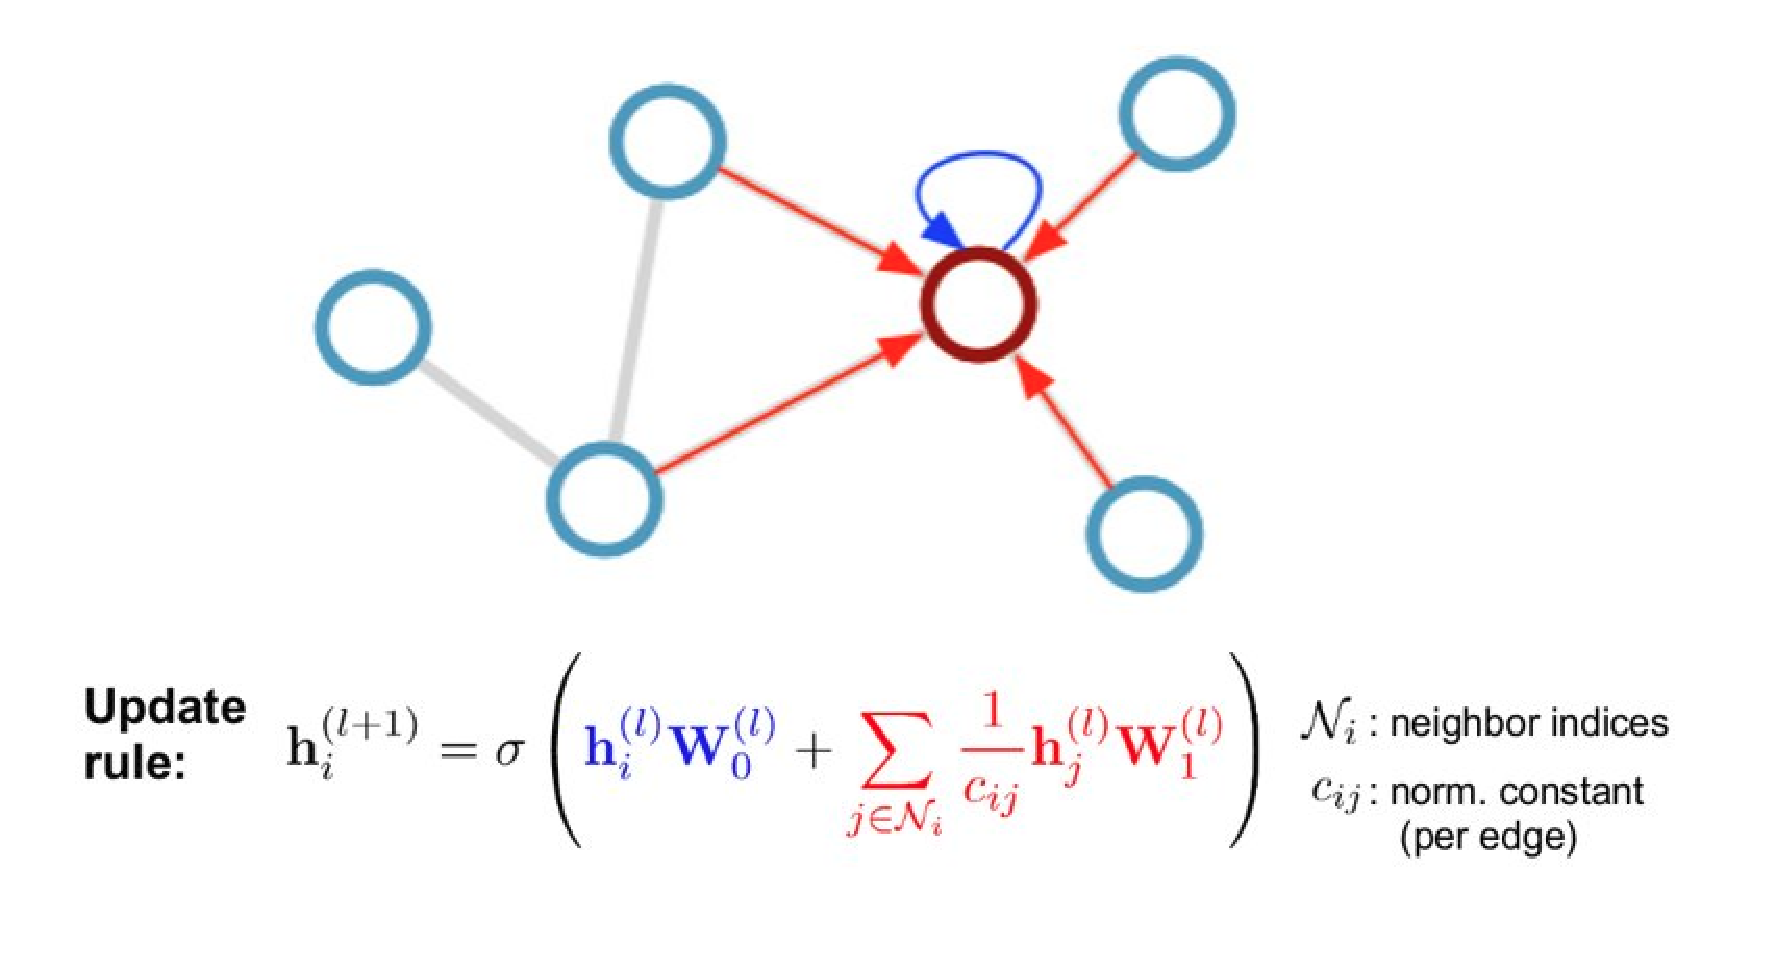
\includegraphics[width=0.7\hsize]{figures/spatial.eps}
  \caption{spatial convolution\cite{gcn}}
  \label{fig:ex1}
\end{figure*}

\section{グラフ畳み込みネットワーク}
$g_{\theta}$をチェビシェフ多項式として近似することにより、spactral convolution を spatial convolutionに近似できるという手法がグラフ畳み込みネットワーク\cite{gcn}である。
グラフ畳み込みネットワークの第$i$層の出力は以下の式で表せる。
\begin{equation}
H^{(i)} = \sigma(D^{-1/2}\tilde{A}D^{-1/2}H^{(i-1)}W^{(i)})
\end{equation}

ここで、$\tilde{A}=A+I_{n}$,$I_{n}\in \mathcal{R}^{n \times n}$は単位行列、$D \in \mathcal{R}^{n \times n}$は次数行列、$H^{(0)}=X$、$W^{(i)}$は$i$層における特徴行列を更新するための重み行列である。また、$\sigma$はReLU関数やsigmoid関数などの活性化関数である。また、教師あり目的関数のロス関数は下の式で更新される。

\begin{equation}
L_{supervised} = - \sum_{l \in y_{l}} \sum_{f=1}^{F} Y_{lf} lnZ_{lf}
\end{equation}
ここで、$y_{l}$はラベル与えられているノード、$Y$はラベル行列、$Z$はグラフ畳み込みネットワーク全体を通しsoftmax関数によって計算される行列である。
この手法はエンドツーエンド学習されている。

\begin{figure*}[h]
  \centering
  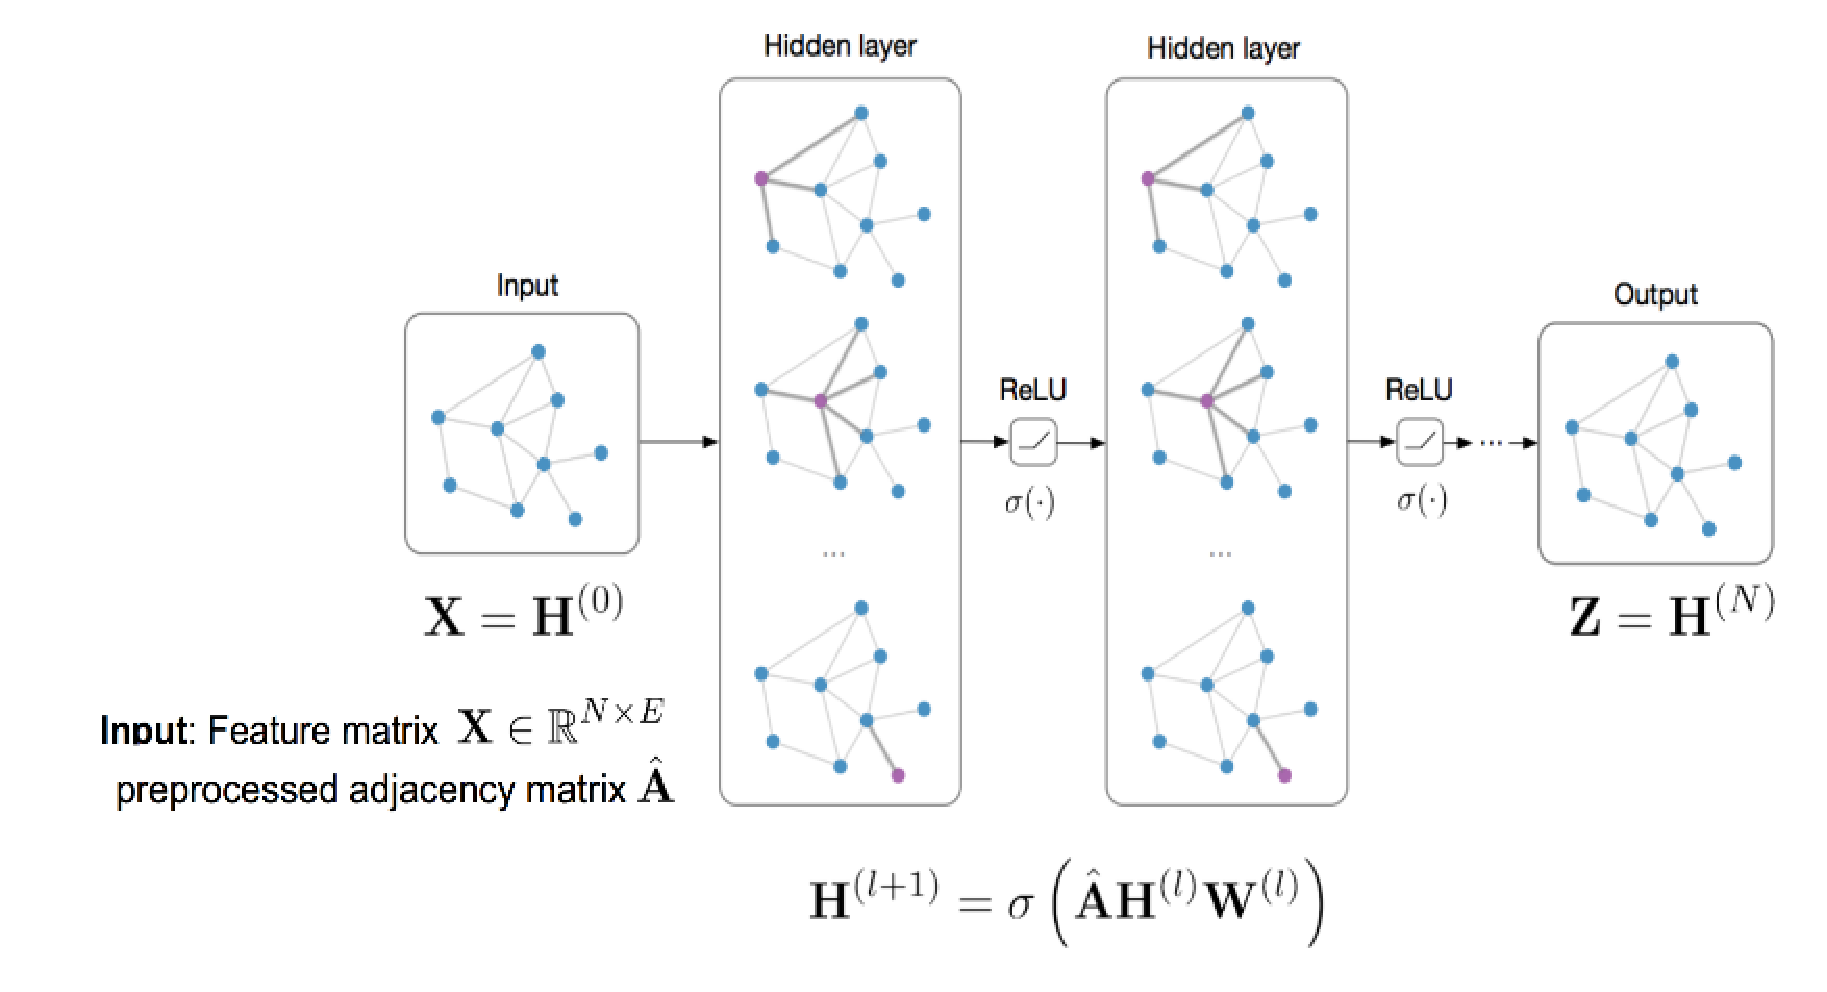
\includegraphics[width=1.0\hsize]{figures/gcn.eps}
  \caption{グラフ畳み込みネットワーク\cite{gcn}}
  \label{fig:ex1}
\end{figure*}





\section{構造特徴}
複雑ネットワークにおいて、そのグラフの特徴を図るための特徴量として構造特徴がある。構造特徴にはグラフ全体を数値で表すグラフ全体構造特徴と、グラフのノードごとを数値で表すノードごとの構造特徴が存在する。
\subsection{グラフ全体の構造特徴}
任意の頂点間の距離の平均を表す平均距離や、グラフ全体におけるエッジによりできたクラスタ(三角形)の個数により定まるクラスター係数などがある。また、これらはグラフ全体において1つの値しか持たないため、ノード分類においてこの特徴量を利用することは難しい。

\subsection{ノードごとの構造特徴}
これらは、グラフにおいて、ノードごとに一つの値が決定されるため、ノード分類の分野に適応しやすい特徴量である。
\begin{itemize}
\item 媒介中心性\\
ノードiが任意のノードペアの最短経路にどれだけ含まれているかを表す指標である。
$$C_i = \frac{\sum_{j<k} path_{jk}(i)/path_{jk}}{(N-1)(N-2)} $$
$path_{jk}$はノードj, k間の最短経路の総数,$path_{jk}(i)$は
その中でノード $i$ を経路に含む最短パスの総数である。
\item 近接中心性\\
ノード$v_{i}$の近接中心性は,ノード$v_{i}$から他のノードまでの平均距離によって定義される。平均的に他のノードに近いほど値は大きくなる。
$$C_i = \frac{N-1}{\sum_j d(v_i,v_j)} $$

\item 次数中心性\\
グラフにおいての他のノードとどの程度直接つながっているのかを表す指標である。$k_{i}$をノード$i$に直接張られたエッジの総数であるとすると ノード$i $の中心性$C_{i}$は以下である。
$$C_i = \frac{k_{i}}{N-1} $$

\item 固有ベクトル中心性\\
ノード$v_{i}$の固有ベクトル中心性は、ノード$v_{i}$と隣接したノードがどれだけ中心性をもっているかという指標である。
$$C_i = \sum_{j} A_{ij} C_j $$
$A_{ij}$は隣接行列の要素である。ノードiからノードjにエッジが張られていたら1,そうでなければ0である。この式の繊維を繰り返し最終的に収束する値$C_i$が求める中心性となる。

\item PageRank\cite{pagerank} \\
pagerankはweb検索に用いられる手法であり、評価の高いページからリンクが多く張られるほどよいページであるというアルゴリズムを用いた手法である。
$$ PR(A) = (1-d) + d \sum_{i=1}^{n} \frac{PR(T_{i})}{C(T_{i})}$$
ここで、$PR(T_{i})$はノード $i$に直接エッジを張っているノードの重要度,$C(T_{i})$はノード$i$に張られたエッジの総数である。dはトレードオフパラメータである。
\end{itemize}
% 上記の他にも,HITS,Katz中心性,フロー中心性,ボナチッチ中心性など,数多くの指標が存在する.

\section{attentionメカニズム}
近年、attentionメカニズムというモデルを使った手法\cite{bahdanau2014neural}\cite{attention}が機械翻訳の分野において高い精度を出し注目を浴びている。attentionメカニズムの一つのやり方として、ベクトル内積を用いて二つのものの類似度をとることにより、必要な情報により多くの注意を払うものである。
例えば下図のように、attentionメカニズムとは自然言語処理の分野において、'making'というqueryが与えられた時に'more'や'difficult'というkey-valueがそのqueryが注意の重みを大きくしていることが分かる。

\begin{figure*}[h]
  \centering
  \includegraphics[width=0.5\hsize]{figures/attention_mechanism.pdf}
  \caption{attentionを用いたモデル\cite{attention}}
  \label{fig:ex1}
\end{figure*}

\begin{figure*}[h]
  \centering
  \includegraphics[width=1.0\hsize]{figures/attention_visualization.pdf}
  \caption{attentionを用いた単語間関係の可視化\cite{attention}}
  \label{fig:ex1}
\end{figure*}
\newpage{}
